\chapter{Diskussion und Ausblick}

Ziel dieser Arbeit ist es, den Schutz der Vertraulichkeit in neuronalen Netzen zu gewährleisten, obwohl sensible Daten genutzt werden. 
Die Vertraulichkeit kann dabei von einer ganzen Reihe an Angriffen bedroht werden.
Kapitel \ref{sec:exp_angriffe} zeigt jedoch, dass weder die Membership Inference Attacke, noch die Model Inversion Attacke effektiv gegen exemplarische Use Cases sind.
Im Folgenden wird deshalb diskutiert, welche Gefahr durch diese Angriffe wirklich entstehen kann.

Außerdem sind neuronale Netze ein aktiver Forschungsbereich. 
Neue Modelle mit neuen Architekturen werden regelmäßig veröffentlicht.
Dies kann dafür sorgen, dass sich auch die Angriffe weiterentwickeln. 
Dies wird ebenfalls im Folgenden betrachtet.

\section{Effektivität der Angriffe}\label{sec:dis_angriffe}
Die Diskussion zur Effektivität der Angriffe basiert auf der Membership Inference Attacke und auf der Model Inversion Attacke, da beide Angriffe in dieser Arbeit bereits evaluiert werden.
Shokri \etal \cite{P-2}, die Forscher, welche die Membership Inference Attacke erstmals vorstellten, zeigen, dass der Angriff effektiv sei, wenn das Modell viele unterschiedliche Klassen vorhersagt und zusätzlich auf die Trainingsdaten overfitted ist.
Overfitting bedeutet, dass ein Modell sehr stark an die Trainingsdaten angepasst ist und deshalb nicht mehr gut generalisiert.
Overfitting zeigt sich, wenn die Genauigkeit auf Trainingsdaten sehr hoch ist, jedoch die Genauigkeit für ungenutzte Daten, wie eine Testdatenmenge, signifikant niedriger ist.
Tabelle \ref{fig:effektivitaet_membership} zeigt die Effektivität der Membership Inference Attacke, welche von Shokri \etal \cite{P-2} evaluiert wurde. 
Die konkreten Use Cases sind dabei zweitrangig. 
Viel wichtiger ist jedoch die Anzahl der Klassen und das Verhältnis zwischen der Genauigkeit gemessen anhand der Trainingsdaten und der Genauigkeit gemessen anhand ungesehener Testdaten.

\begin{table}[!htb]
\centering
\begin{tabular}{lllll}
\hline
\rowcolor[HTML]{CBCEFB} 
\multicolumn{1}{|l|}{\cellcolor[HTML]{CBCEFB}Datenmenge} &
  \multicolumn{1}{l|}{\cellcolor[HTML]{CBCEFB}\begin{tabular}[c]{@{}l@{}}Anzahl an\\ Klassen\end{tabular}} &
  \multicolumn{1}{l|}{\cellcolor[HTML]{CBCEFB}\begin{tabular}[c]{@{}l@{}}Genauigkeit \\ Trainingsdaten\end{tabular}} &
  \multicolumn{1}{l|}{\cellcolor[HTML]{CBCEFB}\begin{tabular}[c]{@{}l@{}}Genauigkeit \\ Testdaten\end{tabular}} &
  \multicolumn{1}{l|}{\cellcolor[HTML]{CBCEFB}\begin{tabular}[c]{@{}l@{}}Effektivität Membership \\ Inference Angriff\end{tabular}} \\ \hline
\multicolumn{1}{|l|}{Einkommen}    & \multicolumn{1}{l|}{2}   & \multicolumn{1}{l|}{84,8 \%}  & \multicolumn{1}{l|}{84,2 \%} & \multicolumn{1}{l|}{50,3 \%} \\ \hline
\multicolumn{1}{|l|}{MNIST}    & \multicolumn{1}{l|}{10}  & \multicolumn{1}{l|}{98,4 \%}  & \multicolumn{1}{l|}{92,8 \%} & \multicolumn{1}{l|}{51,7 \%} \\ \hline
\multicolumn{1}{|l|}{Standort} & \multicolumn{1}{l|}{30}  & \multicolumn{1}{l|}{100,0 \%} & \multicolumn{1}{l|}{67,3 \%} & \multicolumn{1}{l|}{67,8 \%} \\ \hline
                               &                          &                               &                              &                              \\ \hline
\multicolumn{1}{|l|}{Einkauf}  & \multicolumn{1}{l|}{2}   & \multicolumn{1}{l|}{99,9 \%}  & \multicolumn{1}{l|}{98,4 \%} & \multicolumn{1}{l|}{50,5 \%} \\ \hline
\multicolumn{1}{|l|}{Einkauf}  & \multicolumn{1}{l|}{10}  & \multicolumn{1}{l|}{99,9 \%}  & \multicolumn{1}{l|}{86,6 \%} & \multicolumn{1}{l|}{55,0 \%} \\ \hline
\multicolumn{1}{|l|}{Einkauf}  & \multicolumn{1}{l|}{20}  & \multicolumn{1}{l|}{100,0 \%} & \multicolumn{1}{l|}{78,1 \%} & \multicolumn{1}{l|}{59,0 \%} \\ \hline
\multicolumn{1}{|l|}{Einkauf}  & \multicolumn{1}{l|}{50}  & \multicolumn{1}{l|}{100,0 \%} & \multicolumn{1}{l|}{69,3 \%} & \multicolumn{1}{l|}{86,0 \%} \\ \hline
\multicolumn{1}{|l|}{Einkauf}  & \multicolumn{1}{l|}{100} & \multicolumn{1}{l|}{99,9 \%}  & \multicolumn{1}{l|}{65,9 \%} & \multicolumn{1}{l|}{93,5 \%} \\ \hline
\end{tabular}
\caption{Effektivität Membership Inference Attacke nach \cite{P-2}}
\label{fig:effektivitaet_membership}
\end{table}

Der Use Case mit der Datenmenge \dq Einkommen\dq\ besitzt zwei unterschiedliche Klassen und die Genauigkeit anhand der Trainingsdaten ist vergleichbar mit der Genauigkeit der Testdaten.
Es werden also wenige Klasse vorhergesagt und das Modell ist nicht von Overfitting betroffen.
Somit ist die Membership Inference Attacke nicht effektiv, was sich an einer Effektivität von 50,3 \% zeigt.
Ähnlich sieht es bei dem Use Case mit der Datenmenge \dq MNIST\dq\ aus. 
Hier werden 10 Klasse vorhergesagt, wobei die Genauigkeit auf den Testdaten etwas geringer ist, als die Genauigkeit der Trainingsdaten. 
Jedoch ist die Membership Inference Attacke mit 51,7 \% ebenfalls nicht effektiv.
Der Use Case mit der Datenmenge \dq Standort\dq\ unterscheidet zwischen 30 verschiedenen Klassen.
Zusätzlich ist das Modell von Overfitting betroffen, was daran erkennbar ist, dass die Genauigkeit anhand der Trainingsdaten bei vollen 100 \% liegt, die Genauigkeit auf Testdaten lediglich bei 67,3 \%.
Dies sorgt für eine höhere Effektivität der Membership Inference Attacke von 67,8 \%.

Shokri \etal \cite{P-2} evaluieren zusätzlich die Membership Inference Attacke mit der Datenmenge \dq Einkauf\dq, bei welcher die Anzahl an vorhergesagten Klassen bei jedem Modell erhöht wird.
Jedes der Modelle ist von Overfitting betroffen, was an der Genauigkeit erkennbar ist.
Diese liegt bei den Trainingsdaten bei 99,9 \% oder 100,0 \%, wohingegen diese bei den Testdaten geringer ist und bis auf 65,9 \% abfällt.
Die Effektivität des Membership Inference Attacke bei dem Modell, welches 20 Klassen vorhersagt, liegt bei 59,0 \% und ist damit immer noch ineffektiv.
Jedoch sind die Modelle, welche 50 und 100 Klassen vorhersagen, von der Membership Inference Attacke bedroht. 
Bei diesen liegt die Effektivität des Angriffs bei 86,0 \% und 93,5 \%.

Ein weiterer Faktor dieses Angriffs ist es, welche Ressourcen benötigt werden, um diesen Angriff durchzuführen.
Die benötigten Ressourcen hängen primär von der Anzahl der Shadow Modelle ab.
Da jedes Shadow Modell das originale Modell nachahmen soll, ist das Training eines Shadow Modells ressourcentechnisch vergleichbar mit dem des originalen Modells.
Shokri \etal \cite{P-2} nutzen zwischen 10 und 100 Shadow Modellen, was eine Membership Inference Attacke demnach 10 bis 100 Mal so ressourcenintensiv macht, wie das Training des originalen Modells.

Das Handlungsmodell aus Kapitel \ref{ch:handlungsmodell} empfiehlt, die Membership Inference Attacke nur bei streng vertraulichen Daten zu evaluieren. 
Dies liegt an den benötigten Ressourcen, um die Evaluierung durchzuführen.
Der Aufwand, den Angriff bei Daten mit einer niedrigen Vertraulichkeitsklassifizierung zu evaluieren, ist zu hoch.
Dies liegt außerdem daran, dass Overfitting bei jedem Modell nach Möglichkeit vermieden werden soll, was die Membership Inference Attacke ineffektiver macht.

Die Model Inversion Attacke, beziehungsweise die Reconstruction Attacke wurde von Fredrikson \etal \cite{P-3} vorgestellt. 
Kapitel \ref{sec:model_inversion} beschreibt, wie das Bild einer Person rekonstruiert werden kann.
Zur Evaluierung nutzten Fredrikson \etal \cite{P-3} einen Datenbestand, welcher jeweils 10 Bilder von 40 unterschiedlichen Personen zeigt \cite{att}.
Demnach hat jede klassifizierbare Person lediglich 10 Bilder, wobei diese Bilder ähnlich aussehen.
Abbildung \ref{fig:mi_attacke} zeigt, wie das Bild einer Person rekonstruiert wurde. 
Jedoch könnte das rekonstruierte Bild auch ein anderes Bild dieser Person zeigen, da die Trainingsbilder der gleichen Person ähnlich sind.
Ein Indiz für diese Vermutung ist der Mund des rekonstruierten Bildes. 
Im rekonstruierten Bild ist der Mund geöffnet, wohingegen in dem dargestellten originalen Bild der Mund geschlossen ist.
Abbildung \ref{fig:model_inversion_example} zeigt das rekonstruierte Bild von Fredrikson \etal \cite{P-3} mit mehreren Datensätzen der Trainingsdatenmenge.

\begin{figure}[!htb]
\centering
\begin{subfigure}[h]{0.18\textwidth}
  \centering
  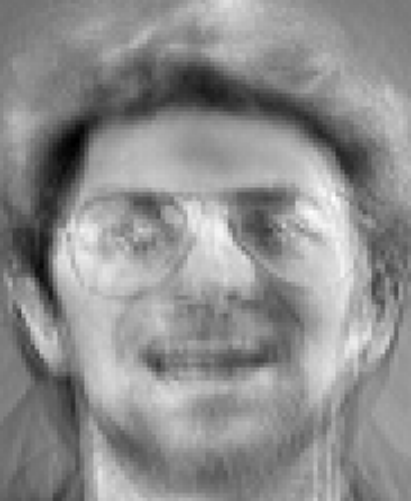
\includegraphics[width=2.58cm]{figures/att/rec.png}
\end{subfigure}
\begin{subfigure}[h]{0.18\textwidth}
  \centering
  
\includegraphics[width=\linewidth]{figures/att/64_7.jpg}
\end{subfigure}
\begin{subfigure}[h]{0.18\textwidth}
  \centering
  
\includegraphics[width=\linewidth]{figures/att/65_7.jpg}
\end{subfigure}
\begin{subfigure}[h]{0.18\textwidth}
  \centering
  
\includegraphics[width=\linewidth]{figures/att/70_7.jpg}
\end{subfigure}
\caption{Mögliche rekonstruierte Datensätze einer Model Inversion Attacke \cite{P-3} \cite{att}}
\label{fig:model_inversion_example}
\end{figure}

Das neuronale Netz, welches die Klassifikation vornimmt, besteht dabei aus drei vollständig verbunden Schichten, wobei die erste Schicht die Eingabeschicht ist und die letzte Schicht die Ausgabeschicht. 
Somit gibt es nur eine Hidden Layer. 
Es werden auch keine Faltungsschichten oder andere komplexere Techniken genutzt.
Die Ähnlichkeit und die geringe Anzahl von Trainingsbildern, sowie eine simple Modellarchitektur sind demnach zwei mögliche Erklärungsmöglichkeiten für die Effektivität der Model Inversion Attacke.

Die Modell Inversion Attacke in Kapitel \ref{sec:exp_angriffe}, evaluierte den Angriff anhand des CIFAR-10 Datenbestand und des CelebA Datenbestands.
Jede Klasse des CIFAR-10 Datenbestands hat 6000 unterschiedliche Bilder \cite{cifar10}, wobei die Bilder selbst mehr Unterschiede aufweisen, als der von Fredrikson \etal genutzte Datenbestand.
Dies liegt daran, dass die Bilder farbig sind und die Objekte in unterschiedlichen Situationen darstellen.
Der CelebA Datenbestand zeigt ebenfalls nur Gesichter an, jedoch gibt es für jedes Merkmal mindestens 4547 Beispiele im Trainingsdatenbestand \cite{celeba}.
Sowohl das Modell für den CIFAR-10 Datenbestand, als auch die beiden Modelle für den CelebA Datenbestand waren deutlich komplexer als das Modell von Fredrikson \etal \cite{P-3}.


Die Erweiterung der Model Inversion Attacke von Zhang \etal \cite{P-4} verbessert den Autoencoder und zeigt den Angriff, wenn ein Angreifer bereits einen Teil des Datensatzes, \zB einen Bildausschnitt, besitzt.
Zhang \etal \cite{P-4} evaluierten den Angriff auf dem CelebA Datenbestand, welcher auch in Kapitel \ref{sec:exp_angriffe} genutzt wird.
Den Autoren gelingt es, fehlende Bildausschnitte eines Datensatzes mit dem Angriff zu befüllen.
Dabei werden auch komplexere neuronale Netze genutzt.

Da es sich bei der Model Inversion Attacke um einen White-Box Angriff handelt, empfiehlt das Handlungsmodell aus Kapitel \ref{ch:handlungsmodell} diesen Angriff nur zu evaluieren, wenn das ganze Modell veröffentlicht wird.
Um den Angriff bestmöglich zu evaluieren, sollte auch Fälle getestet werden, bei denen der Angreifer über Hintergrundwissen oder Teile von Datensätzen verfügt.


\section{Weiterentwicklung von Angriffen durch moderne Modelle}

ChatGPT ist ein Large Language Modell, welches eine Vielzahl von Aufgaben übernehmen kann.
Die Generierung von Bildern gehört bislang nicht dazu.
Jedoch hat OpenAI, das Unternehmen hinter ChatGPT, ein anderes Modell, welches dies kann.
Dieses heißt DALL-E. 
DALL-E 2 ist seit 2022 verfügbar und die neuste Version, DALL-3, wird planmäßig im Oktober 2023 veröffentlicht\footnote{https://openai.com/dall-e-3}.
DALL-E 3 wird voraussichtlich in die ChatGPT Anwendung integriert werden.
Stable Diffusion, \bzw Stable Diffusion XL\footnote{https://stability.ai/blog/stable-diffusion-sdxl-1-announcement}, ist eine Open-Source Alternative zu DALL-E.

Sowohl DALL-E als auch Stable Diffusion erzeugen aus einer Texteingabe ein hochauflösendes Bild.
Die Texteingabe kann dabei den Inhalt des Bildes, als auch den Stil von diesem beschreiben.
Um das Bild zu erzeugen, wird die Texteingabe zuerst in einen latenten Vektorraum konvertiert \cite{stable_diffusion_explained}. 
Diese Konvertierung erfolgt mittels eines Sprachmodells.
Dieser Vektor wird anschließend mittels eines neuronalen Netzes zu einem Bild hochskaliert.
Die Hochskalierung entspricht dabei dem Decoder eines Autoencoders \cite{stable_diffusion_explained}.
Stable Diffusion wurde auf dem LAION-5B Datenbestand trainiert, welcher 5,85 Milliarden Bilder mit einer zugehörigen Beschreibung enthält \cite{laion}.
Sowohl DALL-E als auch Stable Diffusion können qualitativ hochwertige und hochauflösende Bilder erzeugen.
Abbildung \ref{fig:stable_diff} zeigt vier Bilder, welche von Stable Diffusion XL generiert sind\footnote{https://clipdrop.co/stable-diffusion}. Die zugehörige Texteingabe lautet: 
\dq\textit{Panda bear eating a bowl of japanese ramen in an anime style}\dq.

\begin{figure}[!htb]
\centering
\begin{subfigure}[h]{0.22\textwidth}
  \centering
  
\includegraphics[width=\linewidth]{figures/stable_diff/p4.jpg}
\end{subfigure}
\begin{subfigure}[h]{0.22\textwidth}
  \centering
  
\includegraphics[width=\linewidth]{figures/stable_diff/p2.jpg}
\end{subfigure}
\begin{subfigure}[h]{0.22\textwidth}
  \centering
  
\includegraphics[width=\linewidth]{figures/stable_diff/p3.jpg}
\end{subfigure}
\begin{subfigure}[h]{0.22\textwidth}
  \centering
  
\includegraphics[width=\linewidth]{figures/stable_diff/p1.jpg}
\end{subfigure}
\caption{Stable Diffusion XL Beispiele}
\label{fig:stable_diff}
\end{figure}

Diese Modelle zeigen, wozu moderne generative Modelle in der Lage sind.
Diverse Angriffe, wie beispielsweise die Model Inversion Attacke, nutzen ebenfalls generative Modelle. 
Dies ermöglicht verbesserte Versionen des Angriffs.
Beispielsweise könnte die Hochskalierung einer Model Inversion Attacke nicht mehr von einem eigens trainierten Autoencoder übernommen werden, sondern von einem riesigen, öffentlichen Modell wie Stable Diffusion.
Zusätzlich könnten auch neue Arten von Angriffen entwickelt werden.
Eine denkbare Alternative einer Model Inversion Attacke ist es, mittels Stable Diffusion Bilder zu erzeugen, welche vom anzugreifenden Modell klassifiziert werden. 
Die Vorhersagewahrscheinlichkeiten des anzugreifenden Modells können anschließend genutzt werden, um die Eingabetexte von Stable Diffusion iterativ anzupassen.
Dies wird so lange wiederholt, bis das Modell die gewünschte Klasse vorhersagt.
Dabei handelt es sich um einen hypothetischen Angriff, welcher aktuell noch nicht erforscht ist.

Generell besteht das Risiko, dass Fortschritte in der Forschung von neuronalen Netzen dafür sorgen, dass neue Angriffe entstehen und bestehende Angriffe optimiert werden.
Wird beispielsweise eine automatische Evaluierung von Angriffen in einer Deployment-Pipeline eines Modells vorgenommen, sollte darauf geachtet werden, dass aktuelle Angriffe mit fortschrittlichen Angreifermodellen genutzt werden. 

Zusätzlich gibt es die Möglichkeit Penetrationstests von Anwendungen und Infrastruktur auszuweiten oder anzupassen, sodass auch Machine Learning Modelle evaluiert werden.
Dabei werden Angriffe gegen die Vertraulichkeit bei neuronalen Netzen evaluiert, jedoch zusätzlich auch andere Angriffe, welche \zB das Ziel haben, die Güte des Modells zu verschlechtern.
Diese Art von Penetrationstests ist aktuell nicht weit verbreitet, allerdings steigt die Relevanz eines solchen Tests für neuronale Netze.













